% !TEX root =  main.tex

In this section, we give details of computing the Casimir energy via boundary integral operator discretisations. 
Assume 
$\Omega^{-}\in\mathbb{R}^{d}$, for $d \geq 2$ is the interior bounded Lebesgue-measurable domain that the scatterer occupies with piecewise smooth Lipschitz boundary $\Gamma$. The exterior domain is denoted as 
$\Omega^{+} = \mathbb{R}^{d}\backslash\overline{\Omega^{-}}$. $\boldsymbol{n}$ is the exterior unit normal to the surface $\Gamma$ pointing outwards from $\Omega^{-}$ and 
$\boldsymbol{n}_{\boldsymbol{x}}$ is normal to $\Gamma$ at the point $\boldsymbol{x}\in\Gamma$.

In the scalar case, the Casimir energy can be expressed in terms of certain single-layer boundary operator, which we will define below. We then present its relationship with the Krein-Spectral shift function and demonstrate how it can practically be computed.

\subsection{The single-layer boundary operator}
For the bounded interior domain $\Omega^{-}$ or the unbounded exterior domain $\Omega^{+}$, the space of the (locally) square integrable functions is 
\begin{align*}
    L^{2}(\Omega^{-}) &:= \left\{f:\Omega^{\pm}\rightarrow\mathbb{C}, f \text{ is Lebesgue measurable and} \int_{\Omega^{-}}|f|^{2} < \infty \right\},\\
    L_{\text{loc}}^{2}(\Omega^{+}) &:= \left\{f:\Omega^{+}\rightarrow\mathbb{C},\ f \text{ is Lebesgue measurable and} \int_{K}|f|^{2} < \infty, \ \text{for all compact}\ K \subset \Omega^{+} \right\}
\end{align*}
and note that the subscript ``loc'' can be removed if the domain is bounded (i.e. $L_{\text{loc}}^{2}(\Omega^{-}) = L^{2}(\Omega^{-})$).
We define the (local) Sobolev space $H_{\text{loc}}^{s}(\Omega^{\pm})$ as 
\begin{align*}
    H_{\text{loc}}^{s}(\Omega^{\pm}):=\left\{f\in L_{\text{loc}}^{2}(\Omega^{\pm}), \forall\alpha \text{ s.t.} |\alpha|\leq s, D^{\alpha}f\in L_{\text{loc}}^{2}(\Omega^{\pm})\right\},
\end{align*}
where $\alpha = (\alpha_{1}, \alpha_{2}, \dots, \alpha_{d})$ is a multi-index and $|\alpha| = \alpha_{1} + \alpha_{2} + \dots + \alpha_{d}$, and 
the derivative is defined in the weak sense.

For any function $f\in H_{\text{loc}}^1(\Omega)$ we can define the trace $\gamma_{D}^{\pm}$ as
\begin{align*}
    \gamma_{\text{D}}^{\pm}p(\boldsymbol{x}):=\lim_{\Omega^{\pm}\ni\boldsymbol{x'}\rightarrow\boldsymbol{x}\in\Gamma}p(\boldsymbol{x'}).
\end{align*}
We call the range of the trace operator $H^{1/2}(\Gamma)$. This space can be more rigorously defined. But for the purposes of this paper the description of $H^{1/2}(\Gamma)$ is range space of the trace operator is sufficient. We furthermore need the space $H^{-1/2}(\Gamma)$, which is the dual space of $H^{1/2}(\Gamma)$ with $L^2(\Gamma)$ as pivot space.

We can now define the single-layer boundary $\mathcal{V}:H^{-1/2}(\Gamma)\rightarrow H^{1/2}(\Gamma)$ as

\begin{align*}
    (V_{k}\mu)(\boldsymbol{x}) := \int_{\Gamma}g_{k}(\boldsymbol{x},\boldsymbol{y})\psi(\boldsymbol{y})dS_{\boldsymbol{y}}, \ \ \ \ \ 
    \text{for}\ \mu\in H^{-\frac{1}{2}}(\Gamma) \  \text{and} \ \boldsymbol{x}\in\Gamma.
\end{align*}
Here, 
\begin{align}\label{Green's function}
    g_{k}(\boldsymbol{x},\boldsymbol{y}) = \begin{cases}
          \frac{\mathrm{i}}{4}H_{0}^{(1)}(k|\boldsymbol{x}-\boldsymbol{y}|), \ \ \ \ &\text{for} \ d = 2\\
          \frac{e^{ik|\boldsymbol{x}-\boldsymbol{y}|}}{4\pi|\boldsymbol{x} - \boldsymbol{y}|}, \ \ \ \ &\text{for} \ d = 3,
        \end{cases}
\end{align}
with $H_{0}^{(1)}$  a Hankel function of the first kind.



\subsection{Relation between the Krein spectral shift function and the single-layer boundary operator}
By \cite{hanisch2020relative}, the Krein spectral shift function is defined as 
\begin{align*}
    \xi(k) = \frac{1}{2\pi \mathrm{i}}\log\left(\frac{\det(S(k))}{\det(S_{1,k})\cdots\det(S_{N,k})}\right),
\end{align*}
where $S_{i,n}$ is the scattering matrix associated with the $n$th scatterer. These scattering matrices can be constructed  $S_{i,n} = I + 2T_{i,n}$, where 
$I$ is the identity matrix and $T_{i,n}$ is the $T$-matrix. The method of computing the $T$-matrix is fully discussed in \cite{waterman1969new} and 
\cite{ganesh2008far}.

The following theorem links the single-layer boundary operator with the Krein spectral shift function.
\begin{theorem}\cite{hanisch2020relative}
    Consider $\Omega$ as a domain assembling from individual objects $\Omega_{i}$. Let $V_{k}$ be the single-layer boundary operator defined on the boundary 
    $\partial\Omega = \bigcup_{i = 1}^{N}\partial\Omega_{i}$, and $\tilde{V}_{k}$ is the ``diagonal part'' of $V_{k}$ by restricting the integral 
    kernel to the subset $\bigcup_{i = 1}^{N}\partial\Omega_{i}\times\partial\Omega_{i}\subset\partial\Omega\times\partial\Omega$ then the operator 
    $V_{k}\tilde{V}_{k}^{-1}$ is trace-class and 
    \begin{align*}
        \Xi(k) = \log\det\left(V_{k}\tilde{V}_{k}^{-1}\right).
    \end{align*}

    Then for $k > 0$, we have 
    \begin{align*}
        -\frac{1}{\pi}\emph{\text{Im}}\Xi(k) = \frac{\mathrm{i}}{2\pi}(\Xi(k) - \Xi(-k)) = \xi(k)
    \end{align*}
    and by choosing $h(x) = x$ in \eqref{B-K formula}, this gives the formula 
    \begin{align}\label{slp and matrix}
        \emph{\text{Tr}}\left(\Delta^{\frac{1}{2}} + (N - 1)\Delta_{0}^{\frac{1}{2}} - \sum_{i = 1}^{N}\Delta_{j}^{\frac{1}{2}}\right)  = 
        \int_{0}^{\infty}\xi(k)dk = -\frac{1}{\pi}\int_{0}^{\infty}\Xi(\mathrm{i}k)dk.
    \end{align}
\end{theorem}

Equation \eqref{slp and matrix} is used to compute the Casimir energy between the objects and the formula is written as
\begin{align}\label{KSSF and CasE}
    \mathcal{E} = \frac{\hbar c}{2}\int_{0}^{\infty}\xi(k)dk = -\frac{\hbar c}{2\pi}\int_{0}^{\infty}\Xi(\mathrm{i}k)dk
\end{align}

\begin{remark}
    Note that the integral $\frac{\hbar c}{2}\int_{0}^{\infty}\xi(k)dk$ in \eqref{KSSF and CasE} is not Lebesgue convergent and requires regularisation for its numerical evaluation. The right-hand side integral does not suffer from this issue.
\end{remark}

{\color{red} Corrected to here}


\subsection{Galerkin discretization and boundary element spaces}
In order to compute the integral \eqref{KSSF and CasE}, we need to compute the log determinant of the operators $V_{k}\tilde{V}_{k}^{-1}$. In this section we discuss Galerkin discretisations to compute this quantity.

Define the 
triangulation $\mathcal{T}_{h}$ of the boundary surface $\Gamma$ with triangular surface elements $\tau_{l}$ and associated nodes $\boldsymbol{x}_{i}$ 
s.t. $\overline{\mathcal{T}_{h}} = \bigcup_{l}\overline{\tau_{l}}$, where $h$ is the mesh size and define the space of the continuous piecewise linear functions
\begin{align*}
    P_{h}^{1}(\Gamma) = \{v_{h}\in C^{0}(\Gamma): v_{h}|_{\tau_{l}}\in\mathbb{P}_{1}(\tau_{l}), \ \text{for} \ \ \tau_{l}\in\mathcal{T}_{h}\},
\end{align*}
where $\mathbb{P}_{1}(\tau_{l})$ denotes the space of polynomials of order less than or equal to 1 on $\tau_{\ell}$. We have

\begin{align*}
    P_{h}^{1}(\Gamma) := \text{span}\{\phi_{j}\} \subset H^{-\frac{1}{2}}(\Gamma)
\end{align*}
with 
\begin{align*}
    \phi_{j}(\boldsymbol{x}_{i}) = \begin{cases}
        1, & i = j,\\
        0, & i\neq j
    \end{cases}
\end{align*}
being the nodal basis functions.

\begin{remark}
Since $H^{-1/2}(\Gamma)$ does not require continuity we could use a space of simple piecewise constant functions. The reason why we choose piecewise linear functions is the size of the arising matrix systems for dense calculations. The computation of the log-determinant requires $\mathcal{O}(n^3)$ operations, where $n$ is the dimension of our approximation basis. For sphere-like and other similar geometries there are in practice roughly twice as many triangles as nodes in the mesh. Hence, while the assembly cost with piecewise linear functions is higher, the resulting matrix has only half the dimension, resulting in roughly a factor eight reduction of computational complexity for the log determinant. A disadvantage is that on geometries with corners or edges the converges close to these singularities is suboptimal with continuous piecewise linear functions.
\end{remark}

Having defined the basis function $\phi_j$, we can represent each element inside the Galerkin discretization form. Assume there are $N$ objects,
then the matrix of the operator $V_{k}$ is an $N$ by $N$ block matrix, written as 
\begin{align}\label{matrix V}
    \mathsf{V}(k) = \begin{bmatrix}
        \mathsf{V}_{11}(k) & \mathsf{V}_{12}(k) & \cdots & \mathsf{V}_{1N}(k) \\
        \mathsf{V}_{21}(k) & \mathsf{V}_{22}(k) & \cdots & \mathsf{V}_{2N}(k) \\
        \vdots & \vdots & \ddots & \vdots \\
        \mathsf{V}_{N1}(k) & \mathsf{V}_{N2}(k) & \cdots & \mathsf{V}_{NN}(k) \\
\end{bmatrix}
\end{align}
and the matrix $\tilde{V}_{k}$ is the diagonal part of $V_{k}$:
\begin{align}\label{matrix tilde V}
    \tilde{\mathsf{V}}(k) = \begin{bmatrix}
        \mathsf{V}_{11}(k) & 0      & \cdots & 0 \\
    0      & \mathsf{V}_{22}(k) & \cdots & 0\\
    \vdots & \vdots & \ddots & \vdots \\
    0      & 0      & \cdots & \mathsf{V}_{NN}(k) \\
\end{bmatrix}.
\end{align}
Therefore, the element in the $m$th row and $n$th column of the block matrix $\mathsf{V}_{ij}(k)$ is 
\begin{align}\label{Elements in matrix V}
    \mathsf{V}_{ij}^{(m,n)} (k) = \langle V_{ij}(k)\phi_{m}^{(i)}, \phi_{n}^{(j)}\rangle = 
    \int_{\Gamma}\overline{\phi_{m}^{(j)}}(\boldsymbol{x})\int_{\Gamma}g_{k}(\boldsymbol{x}, \boldsymbol{y})\phi_{n}^{(i)}(\boldsymbol{y})dS_{\boldsymbol{y}}dS_{\boldsymbol{x}},
\end{align}
where $\boldsymbol{\phi}^{(i)} = \begin{bmatrix}
    \phi_{1}^{(i)} & \phi_{2}^{(i)} & \dots & \phi_{N}^{(i)}
\end{bmatrix}$ is the set of basis functions defined on the $i$th object and 
\begin{align*}
    \langle f, g \rangle = \int_{\Gamma}{f(\boldsymbol{x})}\overline{g(\boldsymbol{x})}dS_{x}
\end{align*}
denotes the standard $L^{2}(\Gamma)$ inner product.


The value of $\Xi(\mathrm{i}k)$ = $\log\det(V(ik)\tilde{V}(ik)^{-1})$ can be evaluated by computing 
$\log\frac{\det\mathsf{V}(ik)}{\det\tilde{\mathsf{V}}(ik)}$, which is the integrand of the Casimir formula \eqref{KSSF and CasE}. The integrand $\Xi(\mathrm{i}k)$ has a nice numerical property that simplifies the numerical integration, namely it decays exponentially for growing $ik$ along the imaginary axis. While it is possible to demonstrate this decay from analytical properties of the KSSF, in the following we give a simple argument based on matrix perturbation theory.

\begin{theorem}

   {\color{red} Result not correct. Needs to be worked over.}
    Let $\mathsf{V}(\mathrm{i}k)$ and $\tilde{\mathsf{V}}(\mathrm{i}k)$ be the positive definite block matrices defined in \eqref{matrix V} and \eqref{matrix tilde V} 
    for the case of two scatterers (the case of more than two scatterers can be treated similarly), defined by
    \begin{align*}
        \mathsf{V}(\mathrm{i}k) = \begin{bmatrix}
            \mathbb{V}_{11}(\mathrm{i}k) & \mathbb{V}_{12}(\mathrm{i}k)\\
            \mathbb{V}_{21}(\mathrm{i}k) & \mathbb{V}_{22}(\mathrm{i}k)
        \end{bmatrix} \ \ \text{and} \ \   \tilde{\mathsf{V}}(\mathrm{i}k) = \begin{bmatrix}
            \mathbb{V}_{11}(\mathrm{i}k) & 0\\
            0 & \mathbb{V}_{22}(\mathrm{i}k)
        \end{bmatrix}.
    \end{align*} 
    Let $\lambda_i$ be the $i$th eigenvalue of $\mathsf{V}(\mathrm{i}k)$ and correspondingly $\tilde{\lambda}_i$ the $i$th eigenvalue of 
    $ \tilde{\mathsf{V}}(\mathrm{i}k) $, and let $Z$ be the distance between the two scatterers.
    Then, \begin{align*}
        ||\mathsf{V}_{\mathrm{i}k} - \tilde{\mathsf{V}}_{\mathrm{i}k}||_{2} = \mathcal{O}(e^{-Zk})
    \end{align*}
    and the integrand in \eqref{KSSF and CasE} satisfies
    \begin{align}\label{logdet trend}
        \log\frac{\det\mathsf{V}_{\mathrm{i}k}}{\det\tilde{\mathsf{V}}_{\mathrm{i}k}} = \frac{\mathcal{O}(e^{-2Zk})}{\tilde{\lambda}_{\emph{min}}\emph{gap}_{\emph{min}}},
    \end{align}
    where $\tilde{\lambda}_{\emph{min}} = \emph{min}_{i}\tilde{\lambda}_{i}$ and $\emph{gap}_{\emph{min}} = \emph{min}_{i}\emph{gap}_{i}$ with $\emph{gap}_{i}$ defined as 
    \begin{align*}
        \emph{gap}_{i}:= \begin{cases}
            \emph{min}_{\tilde{\lambda}_{j}\in\mathbb{V}_{22}}|\tilde{\lambda_{i}} - \tilde{\lambda_{j}}|, \ \ \emph{if}\ \ \tilde{\lambda}_{i} \in \lambda(\mathbb{V}_{11})\\
            \emph{min}_{\tilde{\lambda}_{j}\in\mathbb{V}_{11}}|\tilde{\lambda_{i}} - \tilde{\lambda_{j}}|, \ \ \emph{if}\ \  \tilde{\lambda}_{i} \in \lambda(\mathbb{V}_{22}).
        \end{cases}
    \end{align*} 
\end{theorem}
\begin{proof}
    By setting $E_{\mathrm{i}k} = \mathsf{V}_{\mathrm{i}k} - \tilde{\mathsf{V}}_{\mathrm{i}k}$, we have 
    \begin{align*}
        ||E_{\mathrm{i}k}||_{2} = \left|\left|\begin{bmatrix}
            0 & \mathbb{V}_{12}(\mathrm{i}k)\\
            \mathbb{V}_{21}(\mathrm{i}k) & 0
        \end{bmatrix}\right|\right|_{2}.
    \end{align*}
    Since the elements in $\mathbb{V}_{12}(\mathrm{i}k)$ and $\mathbb{V}_{21}(\mathrm{i}k)$ are constructed by \eqref{Elements in matrix V} which includes the 
    Green's function $g_{\mathrm{i}k}$ \eqref{Green's function}, we can conclude $||E_{\mathrm{i}k}||_{2} = \mathcal{O}(e^{-Zk})$, where
    $Z$ is the minimal distance between the objects. 

    The bound on the log determinant in  \eqref{logdet trend} is now a consequence of the perturbation bound \cite{MathiasRoy1998QRBf}
    \begin{align}\label{gap}
        |\lambda_{i} - \tilde{\lambda}_{i}| \leq \frac{||E_{\mathrm{i}k}||_{2}^{2}}{\text{gap}_{i}}.
    \end{align}


    Since  $||E_{\mathrm{i}k}||_{2} = \mathcal{O}(e^{-Zk})$, \eqref{gap} becomes $\lambda_{i} - \tilde{\lambda}_{i} = \frac{\mathcal{O}(e^{-2Zk})}{\text{gap}_{i}}$.
    By setting $\tilde{\lambda}_{\text{min}} = \text{min}_{i}\tilde{\lambda}_{i}$ and $\text{gap}_{\text{min}} = \text{min}_{i}\,\text{gap}_{i}$, we have 
    \begin{align*}
        \log\frac{\det\mathsf{V}_{\mathrm{i}k}}{\det\tilde{\mathsf{V}}_{\mathrm{i}k}} &= \sum_{i}\log\frac{\lambda_{i}}{\tilde{\lambda}_{i}}\\
        &= \sum_{i}\log\left[1+\frac{\mathcal{O}(e^{-2Zk})}{\tilde{\lambda}_{i}\text{gap}_{i}}\right]\\
        &= \sum_{i} \frac{\mathcal{O}(e^{-2Zk})}{\tilde{\lambda}_{i}\text{gap}_{i}} + \text{h.o.t}\\
        &\leq \sum_{i}\frac{\mathcal{O}(e^{-2Zk})}{\tilde{\lambda}_{\text{min}}\text{gap}_{\text{min}}} + \text{h.o.t}\\
        &= \frac{\mathcal{O}(e^{-2Zk})}{\tilde{\lambda}_{\text{min}}\text{gap}_{\text{min}}} 
    \end{align*}
\end{proof}
Note that the numerical experiments indicate that the eigenvalues $\{\tilde{\lambda}_{i}\}_{i}$ and the eigenvalue gaps $\{\text{gap}_{i}\}_{i}$ do not exponentially
depend on $k$.


\begin{figure}[H]
    \centering
    \hspace*{-1cm}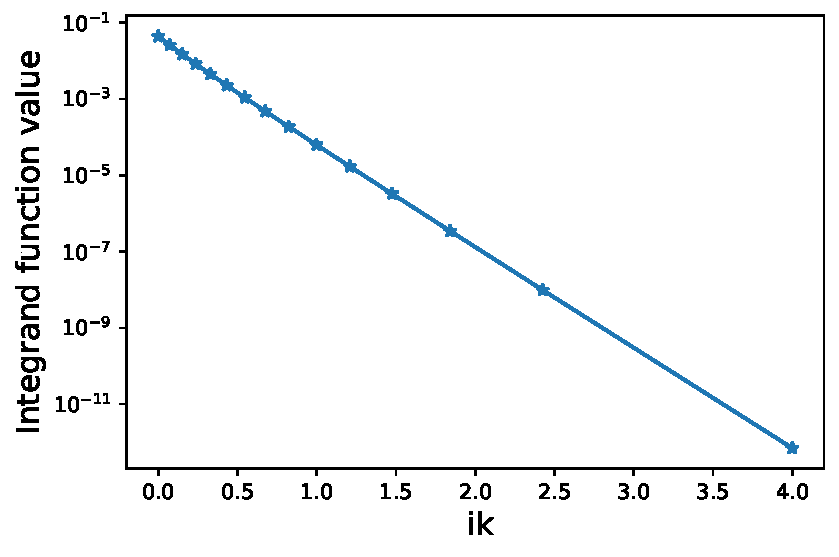
\includegraphics[scale = 0.4]{figures/integ_exp_decay.pdf}
    \caption{(Left) The integrand of the Casimir energy whose value exponentially decays with increasing imaginary wavenumber $\mathrm{i}k$. The integrand function 
    shares the same trend with $e^{-2Zk}$, where $Z$ is the minimal distance between two objects. The scatterers are two spheres with equal radii 
    $R = 1$ with minimal distance $Z = 1.5$. (Right) The integrand of the Casimir energy after changing the 
    variable for applying the trapezoid quadrature rule.}
    \label{The integrand decays exponentially}
\end{figure}


Finally, one can apply the normal trapezoidal rule to calculate the integral 
$\int_{0}^{\infty}\Xi(\mathrm{i}k)dk = \int_{0}^{\infty}\log\frac{\det\mathsf{V}_{\mathrm{i}k}}{\det\tilde{V}_{\mathrm{i}k}}dk$ with variable changed. 
The steps are sketched as follows.

\begin{itemize}
    \item Set $f(k) = \log\frac{\det\mathsf{V}_{\mathrm{i}k}}{\det\tilde{\mathsf{V}}_{\mathrm{i}k}}$ and the range of $k$ is from 0 to $\infty$.
    \item Let $k = -\log(y)$, then the integral $\int_{0}^{\infty}\log\frac{\det\mathsf{V}_{\mathrm{i}k}}{\det\tilde{V}_{\mathrm{i}k}}dk$ becomes 
    $\int_{0}^{\infty}f(k)dk = \int_{0}^{1}\frac{f(-\text{log}(y))}{y}dy$.
    \item Set the range of $k$ as $(\text{lb}, \text{ub})$ \footnote{``ub'' is short for upperbound and ``lb'' is short for lowerbound.} and the corresponding 
    range for $y$ is $(e^{-\text{ub}}, e^{-\text{lb}})\subset[0,1]$.
    \item Choose $m$ quadrature points from the interval $(e^{-\text{ub}}, e^{-\text{lb}})$ and use the trapezoidal rule to evaluate the integral 
    $\int_{e^{-\text{ub}}}^{e^{-\text{lb}}}\frac{f(-\text{log}(y))}{y}dy$. Figure \ref{The integrand decays exponentially} (Right) plots the integrand with regard to new 
    variable $y$($= e^{-k}$).

\end{itemize}



 

